\documentclass[11,]{article}
\usepackage{lmodern}
\usepackage{amssymb,amsmath}
\usepackage{ifxetex,ifluatex}
\usepackage{fixltx2e} % provides \textsubscript
\ifnum 0\ifxetex 1\fi\ifluatex 1\fi=0 % if pdftex
  \usepackage[T1]{fontenc}
  \usepackage[utf8]{inputenc}
\else % if luatex or xelatex
  \ifxetex
    \usepackage{mathspec}
  \else
    \usepackage{fontspec}
  \fi
  \defaultfontfeatures{Ligatures=TeX,Scale=MatchLowercase}
\fi
% use upquote if available, for straight quotes in verbatim environments
\IfFileExists{upquote.sty}{\usepackage{upquote}}{}
% use microtype if available
\IfFileExists{microtype.sty}{%
\usepackage{microtype}
\UseMicrotypeSet[protrusion]{basicmath} % disable protrusion for tt fonts
}{}
\usepackage[margin=1in]{geometry}
\usepackage{hyperref}
\hypersetup{unicode=true,
            pdftitle={The information content of sentiment data from StockTwits},
            pdfauthor={Joyce Cahoon},
            pdfborder={0 0 0},
            breaklinks=true}
\urlstyle{same}  % don't use monospace font for urls
\usepackage{color}
\usepackage{fancyvrb}
\newcommand{\VerbBar}{|}
\newcommand{\VERB}{\Verb[commandchars=\\\{\}]}
\DefineVerbatimEnvironment{Highlighting}{Verbatim}{commandchars=\\\{\}}
% Add ',fontsize=\small' for more characters per line
\usepackage{framed}
\definecolor{shadecolor}{RGB}{248,248,248}
\newenvironment{Shaded}{\begin{snugshade}}{\end{snugshade}}
\newcommand{\AlertTok}[1]{\textcolor[rgb]{0.94,0.16,0.16}{#1}}
\newcommand{\AnnotationTok}[1]{\textcolor[rgb]{0.56,0.35,0.01}{\textbf{\textit{#1}}}}
\newcommand{\AttributeTok}[1]{\textcolor[rgb]{0.77,0.63,0.00}{#1}}
\newcommand{\BaseNTok}[1]{\textcolor[rgb]{0.00,0.00,0.81}{#1}}
\newcommand{\BuiltInTok}[1]{#1}
\newcommand{\CharTok}[1]{\textcolor[rgb]{0.31,0.60,0.02}{#1}}
\newcommand{\CommentTok}[1]{\textcolor[rgb]{0.56,0.35,0.01}{\textit{#1}}}
\newcommand{\CommentVarTok}[1]{\textcolor[rgb]{0.56,0.35,0.01}{\textbf{\textit{#1}}}}
\newcommand{\ConstantTok}[1]{\textcolor[rgb]{0.00,0.00,0.00}{#1}}
\newcommand{\ControlFlowTok}[1]{\textcolor[rgb]{0.13,0.29,0.53}{\textbf{#1}}}
\newcommand{\DataTypeTok}[1]{\textcolor[rgb]{0.13,0.29,0.53}{#1}}
\newcommand{\DecValTok}[1]{\textcolor[rgb]{0.00,0.00,0.81}{#1}}
\newcommand{\DocumentationTok}[1]{\textcolor[rgb]{0.56,0.35,0.01}{\textbf{\textit{#1}}}}
\newcommand{\ErrorTok}[1]{\textcolor[rgb]{0.64,0.00,0.00}{\textbf{#1}}}
\newcommand{\ExtensionTok}[1]{#1}
\newcommand{\FloatTok}[1]{\textcolor[rgb]{0.00,0.00,0.81}{#1}}
\newcommand{\FunctionTok}[1]{\textcolor[rgb]{0.00,0.00,0.00}{#1}}
\newcommand{\ImportTok}[1]{#1}
\newcommand{\InformationTok}[1]{\textcolor[rgb]{0.56,0.35,0.01}{\textbf{\textit{#1}}}}
\newcommand{\KeywordTok}[1]{\textcolor[rgb]{0.13,0.29,0.53}{\textbf{#1}}}
\newcommand{\NormalTok}[1]{#1}
\newcommand{\OperatorTok}[1]{\textcolor[rgb]{0.81,0.36,0.00}{\textbf{#1}}}
\newcommand{\OtherTok}[1]{\textcolor[rgb]{0.56,0.35,0.01}{#1}}
\newcommand{\PreprocessorTok}[1]{\textcolor[rgb]{0.56,0.35,0.01}{\textit{#1}}}
\newcommand{\RegionMarkerTok}[1]{#1}
\newcommand{\SpecialCharTok}[1]{\textcolor[rgb]{0.00,0.00,0.00}{#1}}
\newcommand{\SpecialStringTok}[1]{\textcolor[rgb]{0.31,0.60,0.02}{#1}}
\newcommand{\StringTok}[1]{\textcolor[rgb]{0.31,0.60,0.02}{#1}}
\newcommand{\VariableTok}[1]{\textcolor[rgb]{0.00,0.00,0.00}{#1}}
\newcommand{\VerbatimStringTok}[1]{\textcolor[rgb]{0.31,0.60,0.02}{#1}}
\newcommand{\WarningTok}[1]{\textcolor[rgb]{0.56,0.35,0.01}{\textbf{\textit{#1}}}}
\usepackage{graphicx,grffile}
\makeatletter
\def\maxwidth{\ifdim\Gin@nat@width>\linewidth\linewidth\else\Gin@nat@width\fi}
\def\maxheight{\ifdim\Gin@nat@height>\textheight\textheight\else\Gin@nat@height\fi}
\makeatother
% Scale images if necessary, so that they will not overflow the page
% margins by default, and it is still possible to overwrite the defaults
% using explicit options in \includegraphics[width, height, ...]{}
\setkeys{Gin}{width=\maxwidth,height=\maxheight,keepaspectratio}
\IfFileExists{parskip.sty}{%
\usepackage{parskip}
}{% else
\setlength{\parindent}{0pt}
\setlength{\parskip}{6pt plus 2pt minus 1pt}
}
\setlength{\emergencystretch}{3em}  % prevent overfull lines
\providecommand{\tightlist}{%
  \setlength{\itemsep}{0pt}\setlength{\parskip}{0pt}}
\setcounter{secnumdepth}{0}
% Redefines (sub)paragraphs to behave more like sections
\ifx\paragraph\undefined\else
\let\oldparagraph\paragraph
\renewcommand{\paragraph}[1]{\oldparagraph{#1}\mbox{}}
\fi
\ifx\subparagraph\undefined\else
\let\oldsubparagraph\subparagraph
\renewcommand{\subparagraph}[1]{\oldsubparagraph{#1}\mbox{}}
\fi

%%% Use protect on footnotes to avoid problems with footnotes in titles
\let\rmarkdownfootnote\footnote%
\def\footnote{\protect\rmarkdownfootnote}

%%% Change title format to be more compact
\usepackage{titling}

% Create subtitle command for use in maketitle
\newcommand{\subtitle}[1]{
  \posttitle{
    \begin{center}\large#1\end{center}
    }
}

\setlength{\droptitle}{-2em}

  \title{The information content of sentiment data from StockTwits}
    \pretitle{\vspace{\droptitle}\centering\huge}
  \posttitle{\par}
    \author{Joyce Cahoon}
    \preauthor{\centering\large\emph}
  \postauthor{\par}
    \date{}
    \predate{}\postdate{}
  
\usepackage{placeins}
\usepackage{chngcntr}
\usepackage{multicol}
\usepackage{setspace}
\usepackage{mathrsfs}
\usepackage{amsthm}
\usepackage{graphicx}
\usepackage{booktabs}
\usepackage{multirow}
\usepackage{subcaption}
\usepackage{sidecap}
\usepackage{mathtools}
\usepackage{bm}
\usepackage[linesnumbered,algoruled,boxed,lined,commentsnumbered]{algorithm2e}
\SetKwInput{KwInput}{Input}
\SetKwInput{KwOutput}{Output}
\onehalfspacing
\setlength{\parskip}{8.0pt}
\newcommand{\V}[1]{{\bm{#1}}}
\newcommand{\Real}{\mathbb{R}}
\newcommand{\Exp}{\mathbb{E}}
\newcommand{\ubar}[1]{\underbar{$#1$}}
\newcommand{\obar}{\overline}
\newtheorem{walley781}{Theorem}
\usepackage[symbols,nogroupskip,nonumberlist,automake]{glossaries-extra}
\makeglossaries
\newglossaryentry{T}{name=\ensuremath{T}, description={Number of topics},type=symbols}

\begin{document}
\maketitle
\begin{abstract}
We assessed the performance of a cross-sectional, long-short US equity
strategy that relied soley on sentiment data from StockTwits. Factor
analysis indicates a level of predictive alpha in our sentiment metric
with full exposure five days after the signal is made available in our
portfolio. Our performance over the November 2018 period resulted in a
final rank of 105 out of 261 submissions and a total score of 0.338 on
Quantopia. Its performance is mediocre at best and can be attributed the
fact that the tuning mechanism for input parameters in the algorithm was
based only on the backtest returns. Our results do not yet dismiss the
value of leveraging unstructured data from online conversations to
predict returns.
\end{abstract}

{
\setcounter{tocdepth}{2}
\tableofcontents
}
\newpage

\hypertarget{introduction}{%
\section{Introduction}\label{introduction}}

As fund managers, we were tasked with constructing a cross-sectional,
long-short US equity strategy on
\href{https://www.quantopian.com/}{Quantopian}. There were not many
explicit constraints on the specific strategy we utilized, but it must
pass the following criteria: (i) trade liquid stocks, (ii) have no more
than 5\% of capital invested in any one asset, (iii) have no more than
10\% net dollar exposure, (iv) achieve mean daily turnover between 5\%
and 65\% over a 63-trading-day rolling window, (v) attain gross leverage
between 0.8x and 1.1x, (vi) have low correlation to the market, (vii)
have less than 20\% exposed to each of the 11 sectors as defined on
Quantopian, and (viii) result in positive returns. While the last return
criteria was not a constraint we included in our optimization, we did
design our algorithm with the rest of the seven criteria in mind
(Quantopian \protect\hyperlink{ref-q}{2018}).

The algorithm I eventually submitted was one based purely on the
information content from StockTwits; more specifically, the 5-day moving
average of the bull minus bear intensity associated with each tradable
stock. We rely on this metric to assign each stock's weight in our
portfolio, subject to certain constraints so that our algorithm passes
Quantopian's criteria to remain in competition. Given the large
literature around news and social media sentiment in driving volatility
and liquidity in the market, we wanted to examine the power of this
unstructured data in driving returns.

Our algorithm's performance over the November period resulted in a final
rank of 105 out of 261 submissions and a total score of 0.338. Its
performance is mediocre at best and can be attributed the fact that the
tuning mechanism for my input parameters was based only on the backtest
returns. Given our constraints, e.g.~the length of moving window for our
sentiment metric, were overfit to a backtest window between 2016 and
2018, our strategy may have experienced bad out-of-sample performance.

Nevertheless, this strategy did perform within the top 40\% of all
submissions, which corroborates many findings in literature that social
media has an effect on driving prices. Since the majority of literature
suggests extreme sentiment or extreme volume of online media content
tend to drive returns, and the month of November can be characterized by
extreme volatility, this may explain the high performance of our
sentiment strategy. As expected, for December, the peaks in the VIX
subsided given greater clarity around the Trump administration's trade
policy and Fed's decision to stop raising rates, and our strategy fell a
few ranks to 113 with a score of 0.316 (Gurdus
\protect\hyperlink{ref-cramer2018}{2018}).

\hypertarget{related-work}{%
\section{Related Work}\label{related-work}}

The first paper that explored the relationship of text---unstructured
data---in driving stock prices was Cutler et al.
(\protect\hyperlink{ref-cutler1988}{1988})'s ``What moves stock
prices?'' At the time, the field of computational linguistics was yet
sophisticated enough to process large collections of text, so Cutler and
his team examined 49 major events discussed in the NY Times Business
desk and assessed the market changes associated with each event.
Unfortunately, given the number of significant market moves associated
with days where nothing significant was released, they were unable to
identify any link between market moves and news, possibly stymeing
explorations into this realm (Cutler et al.
\protect\hyperlink{ref-cutler1988}{1988}). Fortunately, another
empirical study emerged in 1998, which leveraged information on online
message boards instead, identifying strong correlations between stocks
with high message volume and high market valuation. In fact, Wysocki
found message volume forecasted not only abnormal stock returns the next
day, but also trading volume the next day (Wysocki
\protect\hyperlink{ref-wysocki1998}{1998}).

Yet, given these results and similar findings from papers like Bagnoli
et al. (\protect\hyperlink{ref-bagnoli1999}{1999}), Antweiler and Frank
(\protect\hyperlink{ref-antweiler2004}{2004}), corroborating the link
between prices and social chatter, a number of studies find the
opposite. Tumarkin and Whitelaw
(\protect\hyperlink{ref-tumarkin2001}{2001}) found no relationship for
equities in the tech sector and the message activity on RagingBull.com.
Das and Chen (\protect\hyperlink{ref-das2007}{2007}) developed a
classifier for investor sentiment from message board text, but was
unable to to demonstrate its ability to forecast returns. Dewally
(\protect\hyperlink{ref-dewally2003}{2003}) found recommendations
exchanged on sites like \texttt{misc.invest.stocks} and
\texttt{alt.invest.penny-stocks} had no effect on the return
characteristics of the stocks under discussion.

Despite these mixed claims, newer studies arose reporting the opposite.
The seminar paper by Tetlock (\protect\hyperlink{ref-tetlock2007}{2007})
concluded high negative sentiment in the Wall Street Journal predicted
temporary downward price pressure, echoing the thoughts expressed in
Wysocki (\protect\hyperlink{ref-wysocki1998}{1998}) that extreme news
affects market movement. Additional works that build on Tetlock's use of
news as a fundamental factor is Mitra et al.
(\protect\hyperlink{ref-mitra2008}{2008}), Leinweber and Sisk
(\protect\hyperlink{ref-leinweber2011}{2011}) and Fang and Peress
(\protect\hyperlink{ref-fang2009}{2009}), each providing evidence for
the predictive value in social chatter. In this class, we were also
directed to the paper by Agrawal et al.
(\protect\hyperlink{ref-agrawal2019}{2019}), which provides a great
overview of literature that further promotes the use of Twitter and
StockTwits to predict stock volatility, liquidity and return.

\hypertarget{stocktwits-data}{%
\section{StockTwits Data}\label{stocktwits-data}}

Key to our strategy is the output from the \texttt{bull\_minus\_bear}
API call as it is this signal that is fed into the optimization function
and this result that determines the order size of each asset. While
there is no disclosure on the natural language processing model that
calculates the bull and bear intensity of each social media message, it
is helpful to look at examples and understand the nature of posts that
ultimately determine the power of our sentiment measure.

\begin{figure}

{\centering 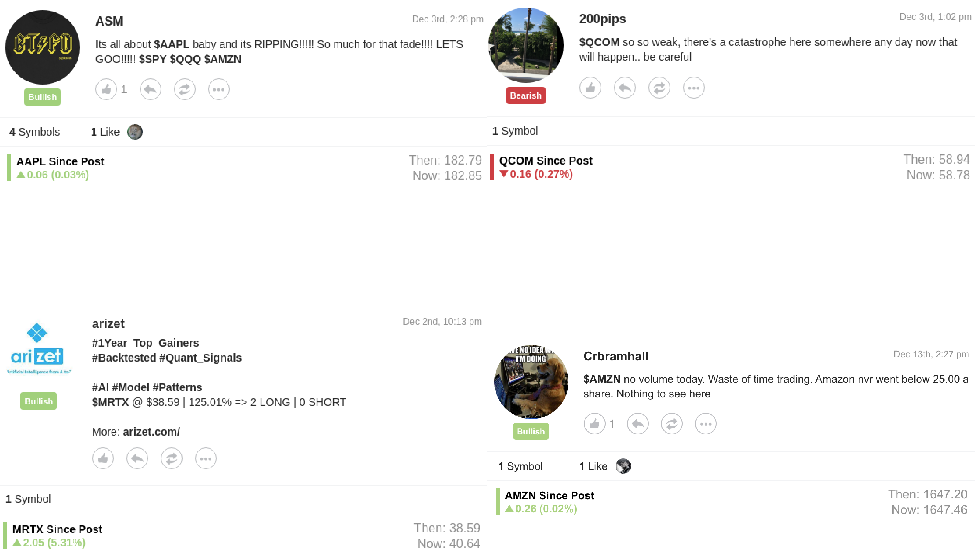
\includegraphics[width=0.8\linewidth]{cahoon_final_paper_files/figure-latex/unnamed-chunk-2-1} 

}

\caption{\label{StockT}Four examples of messages posted on StockTwits. The bull and bear indicator is tagged by the user, and all stock tickers that follow the cashtag symbol is associated with this bull or bear flag. The bull and bear intensity is then computed by a proprietary StockTwits algorithm based on the content within each individual post.}\label{fig:unnamed-chunk-2}
\end{figure}

As shown in Figure \ref{StockT}, there is a lot of noise in StockTwit
data as users each utilize the platform for different reasons and do not
have to disclose any of their personal stakes in the equities they
support. Logically, users that are more influential should have a higher
impact in driving overall investor sentiment, and thus driving prices,
but there currently is no easily available API call that provides such a
weighting. Moreover, these influencers change over time, increasing the
difficulty around identifying posts that might hold more significance
than another. As a result, relying on the aggregate bullish and bearish
intensity averaged daily across all tagged StockTwits messages is the
best surrogate we have to understanding community sentiment for a
specific stock.

From the free version of StockTwits API, we have access to the following
daily metrics for 10,214 liquid US equities (``StockTwits''
\protect\hyperlink{ref-st}{2018}):

\begin{itemize}
\tightlist
\item
  \emph{Bull and bear scored messages}: Total number of daily messages
  that were labeled either ``Bullish'' or ``Bearish'' on the StockTwits
  platform by the user.
\item
  \emph{Bull or bear intensity}: Daily score between 0 and 4 aggregated
  across processed messages. 0 means no bull or bear sentiment was
  detected by StockTwits proprietary trading algorithm. 4 means very
  high bull or bear sentiment was detected. Exploratory data analyses
  indicate that very few stocks receive a score of 4.
\item
  \emph{Total scanned}: Total number of daily messages that appear on
  StockTwits platform that has at least one cashtag associated with it.
  The message is included in this count whether it is labeled or
  unlabeled and whether it can be processed by the StockTwist language
  algorithm or not.
\end{itemize}

Since \emph{disagreement} among message content has been shown to be
associated with greater liquidity and volatility, we focus on the metric
of \texttt{bull\_minus\_bear} as it is one proxy for disagreement among
investor opinion (Antweiler and Frank
\protect\hyperlink{ref-antweiler2004}{2004}). Given the overall trend in
this metric is not stable as we will see in Figure \ref{topstock} and
\ref{botstock}, a moving average is taken. Eventually, we settle on
5-day moving average as the mean information coefficient (IC) is
positive that this point. The IC is often chosen to evaluate whether a
factor is predictive of returns as it is more robust to outliers and
normality assumptions. It allowed us to better tease out whether two
series move in concert or not.

IC was thus calculated from the rank of each data pair in each
series---our intensity difference versus returns---as
\(IC = 1- 6\sum_i d_i^2 / n(n^2-1)\) where \(d_i\) represents the
difference in ranks. As shown in the top left of Figure \ref{IC}, prior
to 5 trading days, our sentiment signal hurts our returns in that its
forecast is negative, but after 5 trading days, we gain some predictive
power. This is further corroborated in the top right plot in that
returns are highest when the signal is delayed by four days. Given the
IC results, we may want to build greater exposure to this factor as it
still benefits us after 10 trading days. We can also leverage the
positive effects of this factor by increasing our turnover constraints
as it appears it does not hurt our portfolio to keep in there for a
longer period of time.

Another asset is that our sentiment factor has relatively low exposures
throughout, with most of the returns from volatility risk. However,
there does appear to be persistent exposure to value and short term
reversal, in that it is shifted to the left of zero; and persistent
exposure to size and momentum, in that it is shifted to the right of
zero. Ideally, we would choose a factor that does not display any skew,
but our skews do not appear that large. We benefit from the fact that
the width of each of our box and whisker plots are not that wide, so our
exposures do not vary much over time.

Unfortunately, when we examine our exposures through cumulative returns
and volatility, we find that our sentiment factor may not be as strong
as we desired. As shown by the bottom left bar graph in Figure \ref{IC},
most of our returns are obtained from exposure to common risk factors,
and, as shown in the right bar graph, are in fact driven by these common
risk factors. Ideally, we would like to strip away the contribution from
these common risk factors as portfolio performance from this exposure
can easily be replicated from ETFs or other easy, cost-effective
methods. Alternatively, we can work to identify asset classes to include
in our portfolio that would offset the exposure risks identified.
Nevertheless, this factor analysis was conducted only over the sentiment
signal in 2018, so there exist other extended periods prior to 2018 in
which our factor may over or underperform.

\begin{figure}

{\centering 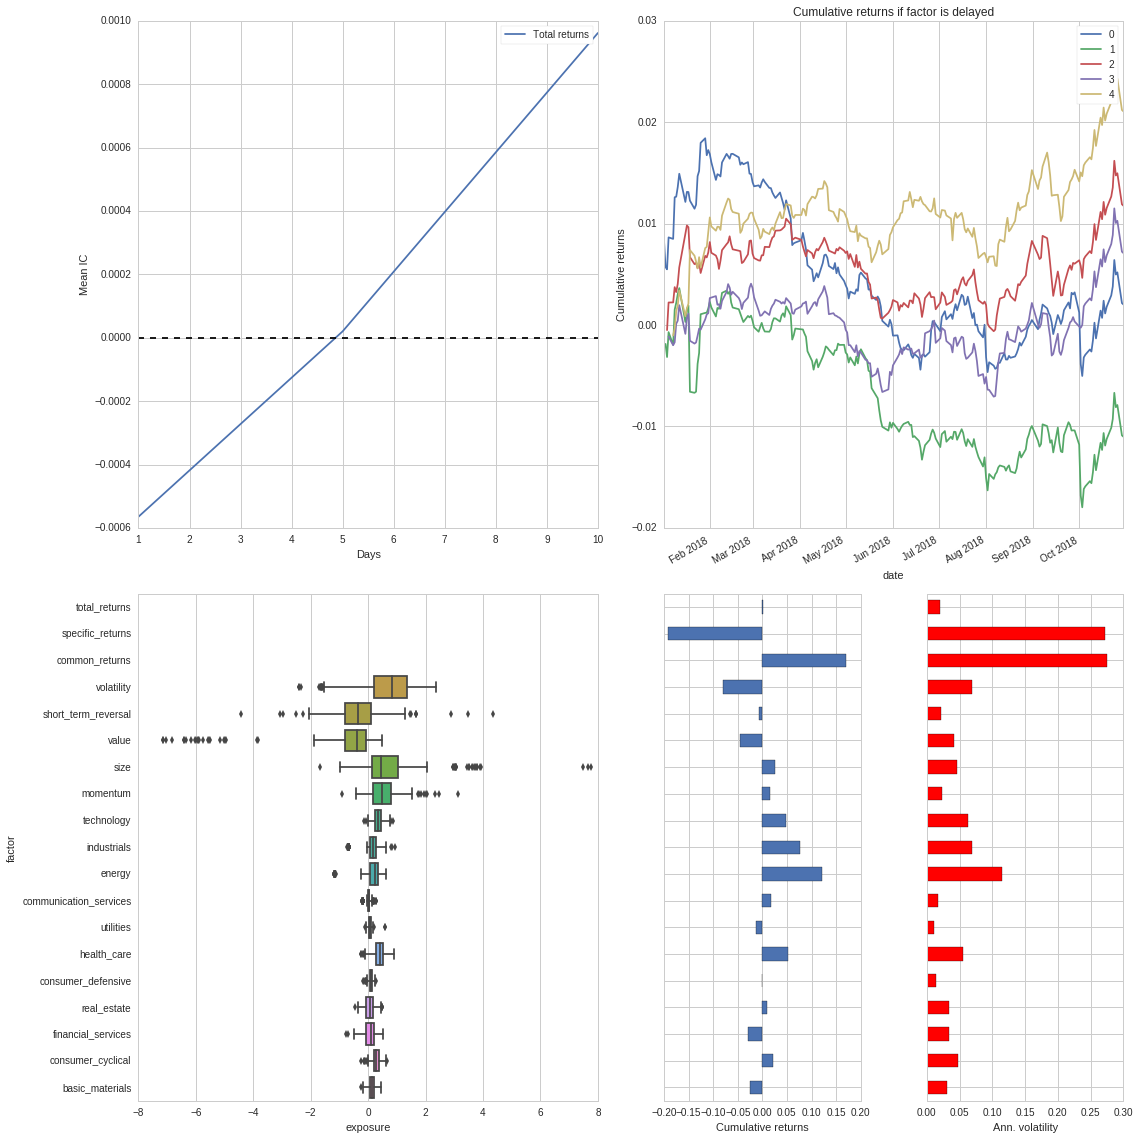
\includegraphics[width=0.8\linewidth]{~/workspace/st790-financial-stats/final/download2} 

}

\caption{\label{IC}Examination of (top-right) information coefficient averaged over all possible asset returns, (top-left) cumulative returns when factor is delayed, (bottom-left) risk exposures, and (bottom-right) cumulative returns and volatility.}\label{fig:unnamed-chunk-3}
\end{figure}

\hypertarget{trading-strategy}{%
\section{Trading Strategy}\label{trading-strategy}}

Given the ease of implementation and some good alpha characteristics as
delineated above, we chose to use the sentiment factor in our trading
strategy. Continuous backtesting was run to derive the constraint
parameters as outlined:

\begin{enumerate}
\def\labelenumi{\arabic{enumi}.}
\tightlist
\item
  We filter a universe of liquid assets from
  \(\texttt{QTradeableStocksUS}\) that pass the following criteria:

  \begin{itemize}
  \tightlist
  \item
    It is not trading within 2 days of earnings as assets are generally
    more volatile within these dates.
  \item
    It has not been announced as an acquisition target to further reduce
    any possible volatility.
  \item
    We are able to calculate a 5-day moving average of the
    bull-minus-bear signal.
  \end{itemize}
\item
  We build an alpha vector for the universe of liquid assets filtered
  from our step above. The alpha model we use is quite simple: we rank
  the assets by its bull-to-bear intensity, averaged over the past 5
  days as evaluated from StockTwits, and find a set of new portfolio
  weights that maximizes the sum of each asset's weight times this alpha
  value. Our objective defined in \texttt{MaximizeAlpha} is thus simply
  a function of this sentiment datastream as we believe this ranking is
  similar to expected returns of each asset. Our routine effectively
  goes long on assets with high bullish signal and short on those with a
  high bearish signal.
\item
  Once a week, we calculate the portfolio that maximizes the
  alpha-weighted sum of our position sizes, subject to the following
  constraints:

  \begin{itemize}
  \tightlist
  \item
    Our portfolio maintains a gross leverage of, or less than, 1.0x.
  \item
    Our portfolio has no more than 5\% in any single asset.
  \item
    Our portfolio does not pass mean daily turnover of 80\%.
  \end{itemize}
\end{enumerate}

Our simple strategy can be summarized as follows:

\[
\max_{{\bm{w}} \in \mathbb{R}^n} {\bm{\alpha}}^T {\bm{w}} \quad \text{subject to} \quad |w_i| \leq 0.05,\; \sum_i |w_i| \leq  1.00, \; \sum_i |w_i-w_{i-1}| \leq 0.80, \; \sum_i w_i = 1
\] \noindent where \({\bm{w}}\) represents the weights attached to each
asset in our optimal portfolio.

\hypertarget{backtest-analysis}{%
\section{Backtest Analysis}\label{backtest-analysis}}

We test our trading strategy with \$10 million in capital from September
30, 2016 to December 3, 2018. Table \ref{bt} outlines our performance
during this period:

\begin{table}[ht]
\centering
\caption{Key metrics from our final backtest between 2016 and 2018.}
\begin{tabular}{lllll}
                                        &                             &                       &                                     &                             \\ \cline{1-2} \cline{4-5} 
\multicolumn{1}{|l|}{Annual Return}     & \multicolumn{1}{l|}{1.7\%}  & \multicolumn{1}{l|}{} & \multicolumn{1}{l|}{Skew}           & \multicolumn{1}{l|}{0.18}   \\ \cline{1-2} \cline{4-5} 
\multicolumn{1}{|l|}{Cumulative Return} & \multicolumn{1}{l|}{3.6\%}  & \multicolumn{1}{l|}{} & \multicolumn{1}{l|}{Gross Leverage} & \multicolumn{1}{l|}{0.99}   \\ \cline{1-2} \cline{4-5} 
\multicolumn{1}{|l|}{Annual Volatility} & \multicolumn{1}{l|}{4.0\%}  & \multicolumn{1}{l|}{} & \multicolumn{1}{l|}{Daily Turnover} & \multicolumn{1}{l|}{18.6\%} \\ \cline{1-2} \cline{4-5} 
\multicolumn{1}{|l|}{Sharpe Ratio}      & \multicolumn{1}{l|}{0.43}   & \multicolumn{1}{l|}{} & \multicolumn{1}{l|}{Alpha}          & \multicolumn{1}{l|}{0.01}   \\ \cline{1-2} \cline{4-5} 
\multicolumn{1}{|l|}{Max Drawdown}      & \multicolumn{1}{l|}{-3.1\%} & \multicolumn{1}{l|}{} & \multicolumn{1}{l|}{Beta}           & \multicolumn{1}{l|}{0.02}   \\ \cline{1-2} \cline{4-5} 
                                        &                             &                       &                                     &                            
\end{tabular}
\label{bt}
\end{table}

While the annualized and cumulative returns are low, at 1.7\% and 3.6\%
respectively, we settle on the parameters in our trading strategy as it
has a number of good properties. For a start, its overall beta of 0.02
is ideal, suggesting low correlation with the market and less
volatility. As shown in Figure \ref{beta}, this overall average is
representative as the rolling beta does not deviate far from this value.

\begin{figure}

{\centering 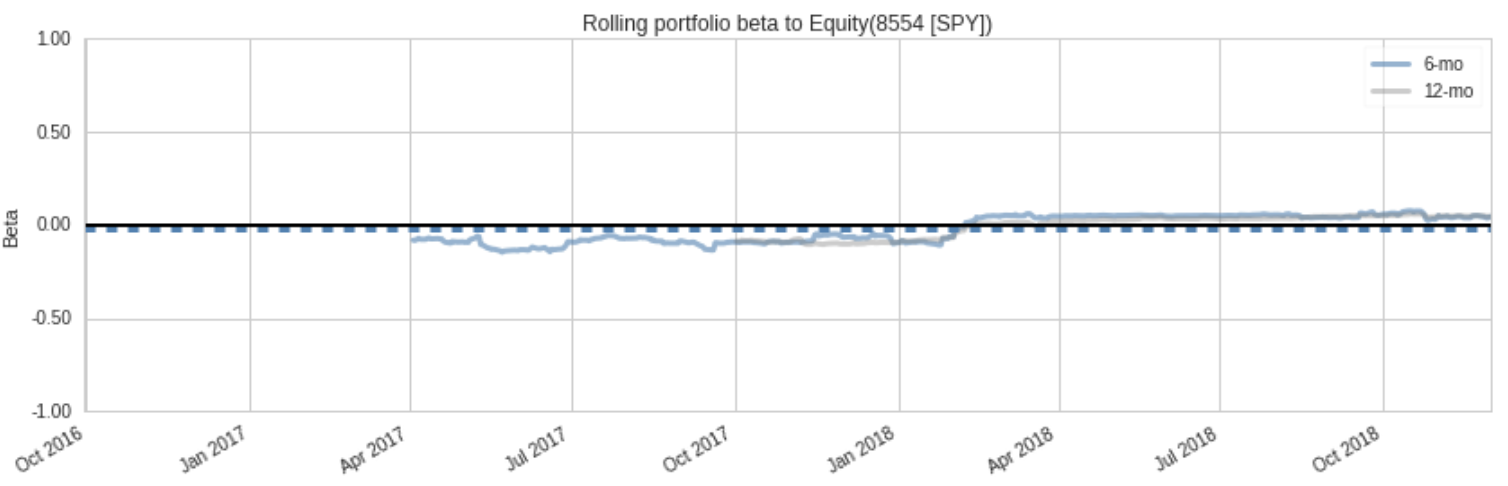
\includegraphics[width=0.8\linewidth]{/Users/jcahoon/workspace/st790-financial-stats/final/ts_rolling_beta} 

}

\caption{\label{beta}Rolling beta calculated within the backtest period suggests the strategy is market neutral.}\label{fig:unnamed-chunk-4}
\end{figure}

Our Sharpe ratio of 0.43 suggests low risk-adjusted return. Generally,
leverage can be applied to such low risk strategies to increase the
absolute return; however, when we examine the Sharpe ratio over our
backtest period, we find high variability. This lack of consistency in
Figure \ref{sharpe} makes our trading strategy much more difficult to
assess.

\begin{figure}

{\centering 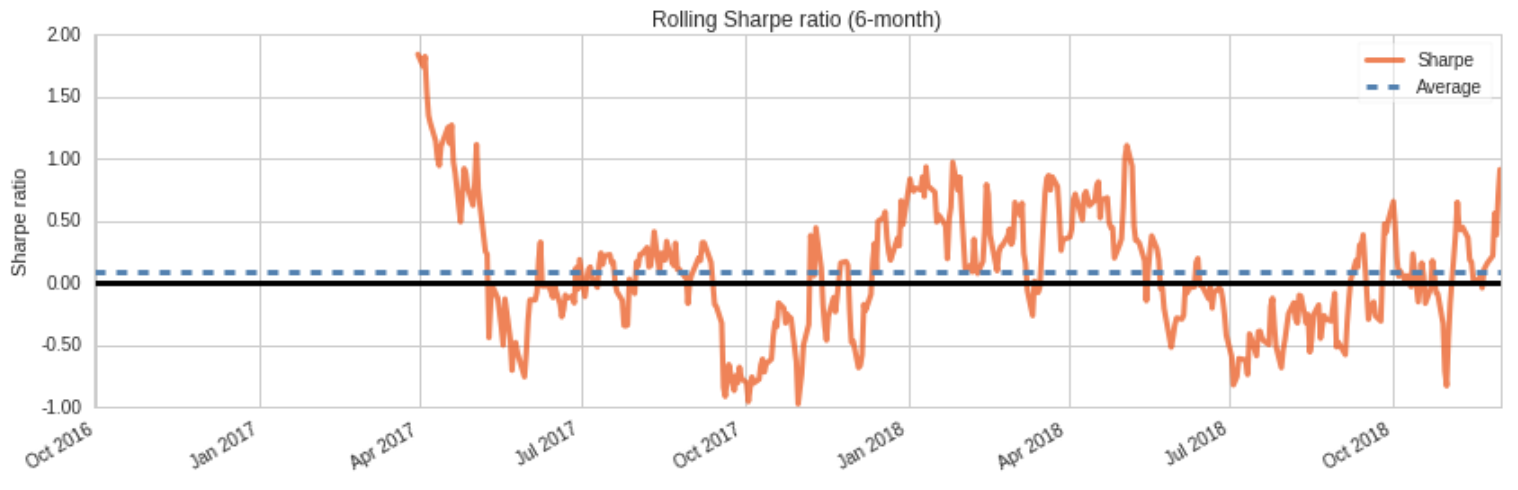
\includegraphics[width=0.8\linewidth]{/Users/jcahoon/workspace/st790-financial-stats/final/ts_rolling_sharpe_ratio} 

}

\caption{\label{sharpe}Rolling Sharpe calculated within the backtest period suggests it is highly inconsistent.}\label{fig:unnamed-chunk-5}
\end{figure}

From our cumulative returns in Figure \ref{cul}, we see our
underperforming Sharpe ratios, within the June 2017 and January 2018
window, as well as the May 2018 and October 2018 window, occur during
periods where the cumulative market returns are increasing at a rate
much higher than that of our portfolio. This makes sense given our
initial exploratory result; our sentiment metric has the highest
exposure to volatility risk.

\begin{figure}

{\centering 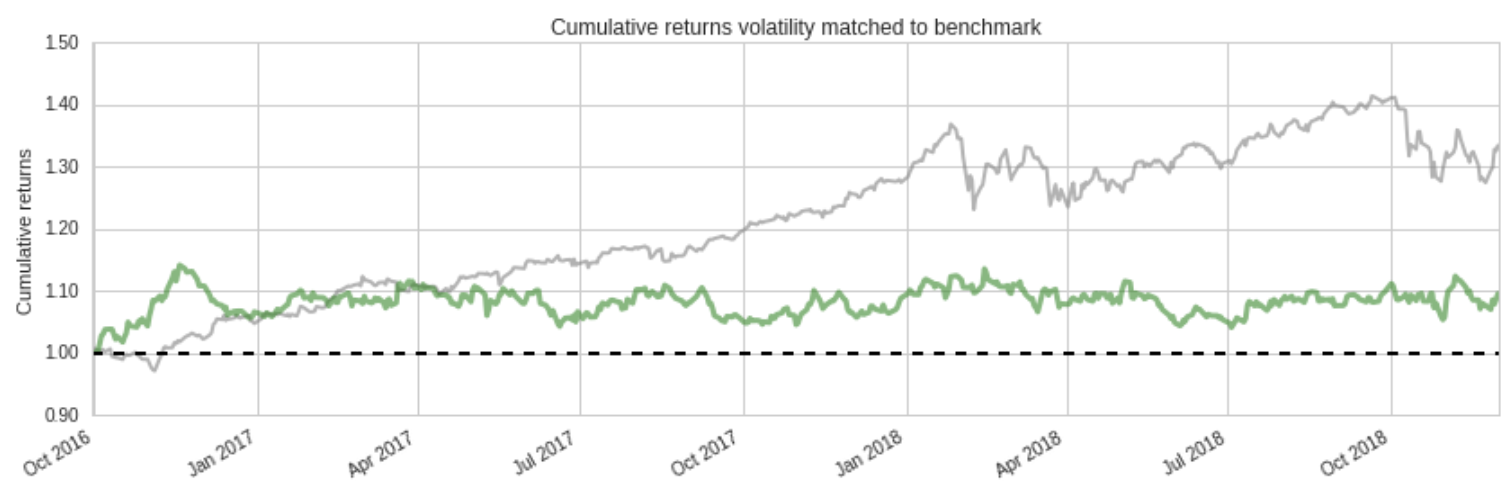
\includegraphics[width=0.8\linewidth]{/Users/jcahoon/workspace/st790-financial-stats/final/ts_cumulative_return_vol} 

}

\caption{\label{cul}Cumulative returns of our portfolio against the market portfolio.}\label{fig:unnamed-chunk-6}
\end{figure}

When we align our rolling Sharpe ratios in Figure \ref{sharpe} against
our underwater plot in Figure \ref{under}, we also find when our
strategy performs worse. It narrows our original windows to months
surrounding the July 2017 and June 2018. Coincidentally, both these
periods are marked by heavy gains in the broader market due to good
macroeconomic news like job gains and high earnings. Given our low beta,
our strategy might result in better performance in times of market
decline.

\begin{figure}

{\centering 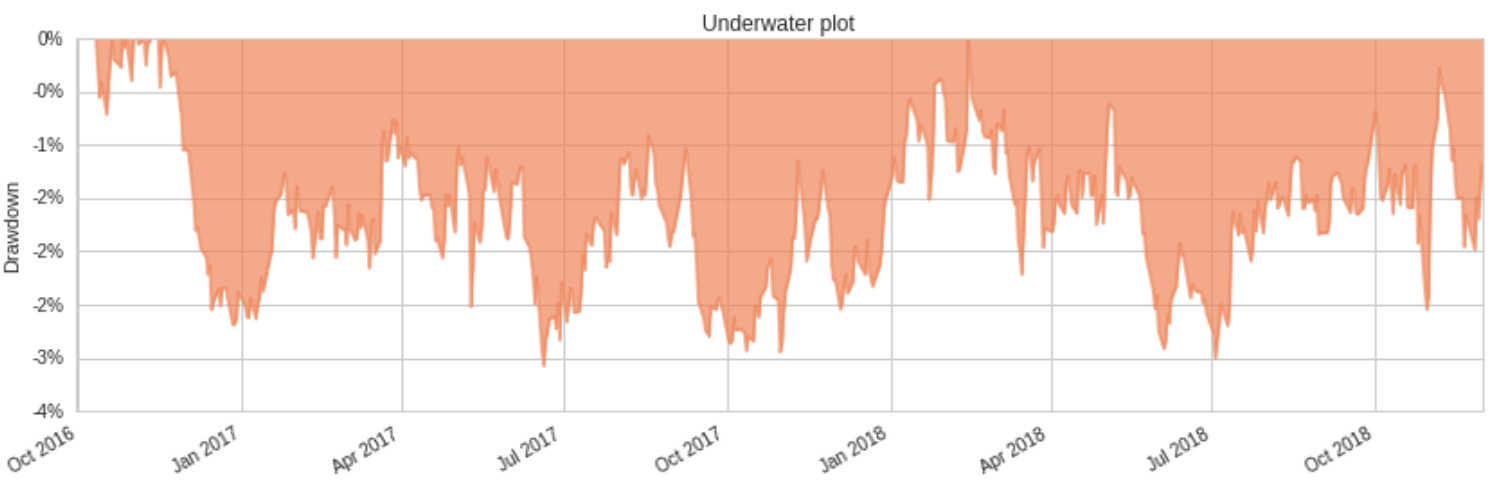
\includegraphics[width=0.8\linewidth]{/Users/jcahoon/workspace/st790-financial-stats/final/ts_underwater} 

}

\caption{\label{under}Underwater plot highlighting periods of max drawdown.}\label{fig:unnamed-chunk-7}
\end{figure}

Overall, our drawdowns are minimal, none surpassing the 4\% mark. We
thus move on to examine whether there is any seasonality to our strategy
in Figure \ref{season}. While it is not explicit, it does appear our
strategy has performed well within the month of November for 2016, 2017
and 2018. The annual returns, however, are quite low in 2017 and 2018
compared to 2016, which could be explained by the traffic on StockTwits
platform. As we will examine further on an individual stock basis, it
appears our bull minus bear intensity is evaluated on very little data.

\begin{figure}

{\centering 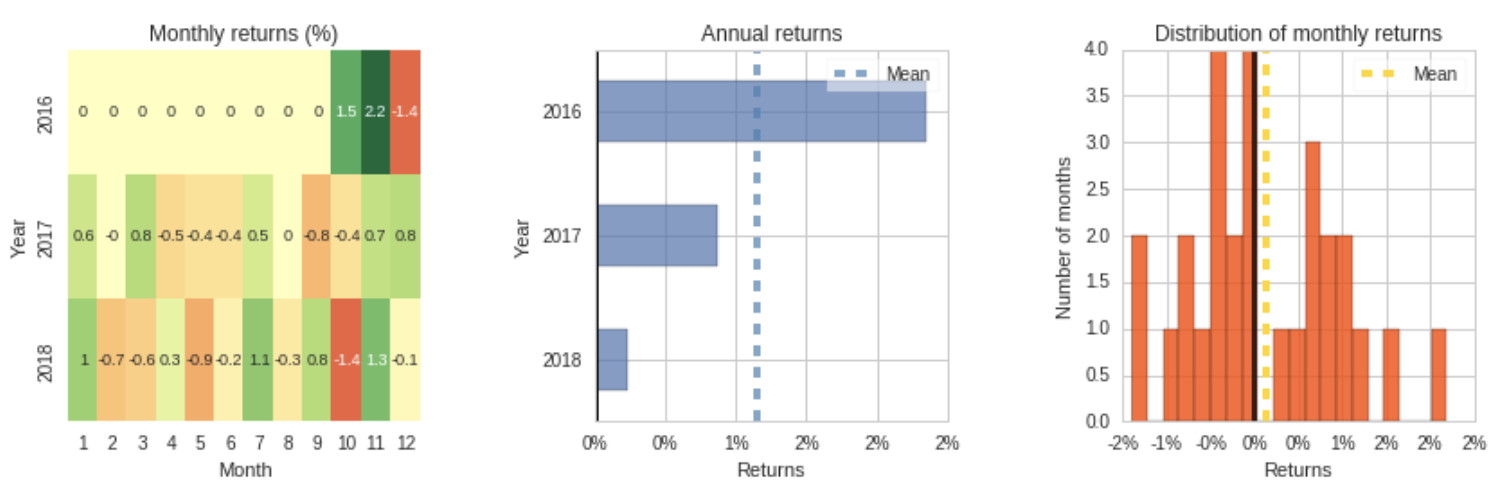
\includegraphics[width=0.8\linewidth]{/Users/jcahoon/workspace/st790-financial-stats/final/ts_seasonal} 

}

\caption{\label{season}(Left) Monthly returns of our overall portfolio broken down by year. (Center) Annual returns. (Right) Histogram of monthly returns.}\label{fig:unnamed-chunk-8}
\end{figure}

As we saw in our exploratory analysis in Figure \ref{IC}, we also see
that we have relatively low exposures to each industry in Figure
\ref{industry}, protecting us from idiosyncratic shocks. We also see in
Figure \ref{leverage} and \ref{turnover} an expected pattern over our
backtest period as we fixed these metrics in our original strategy.

\begin{figure}

{\centering 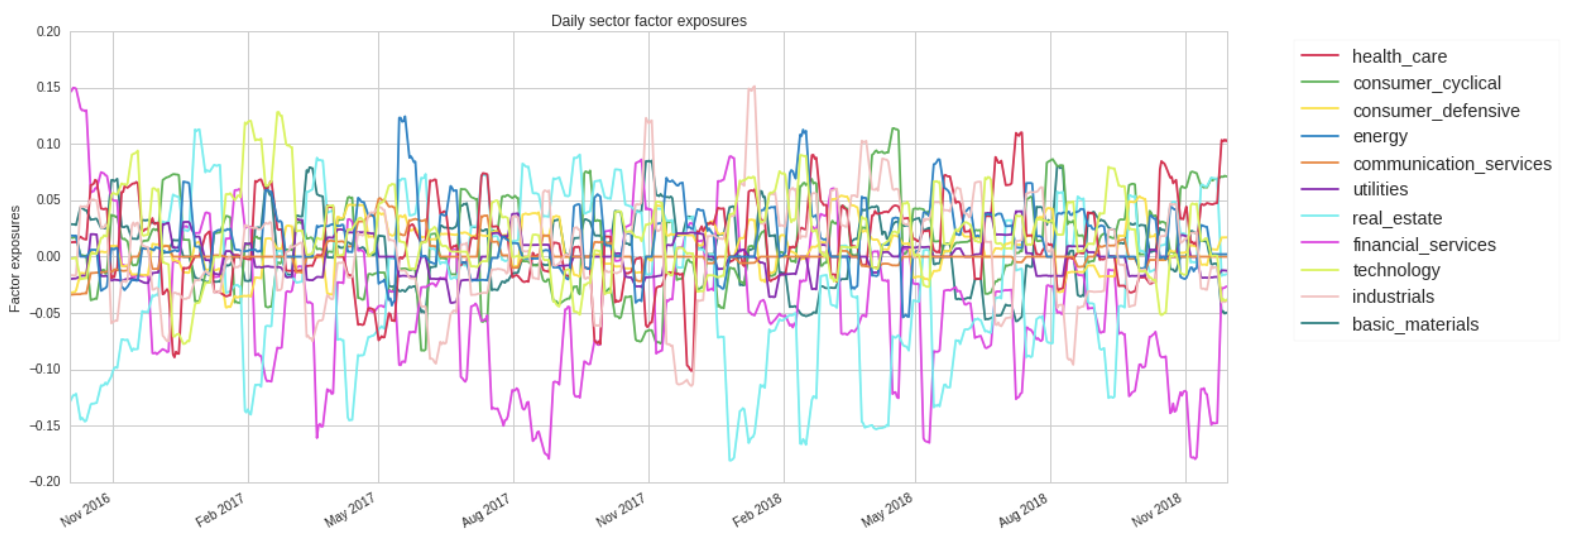
\includegraphics[width=0.8\linewidth]{/Users/jcahoon/workspace/st790-financial-stats/final/ts_daily_factor_exposures} 

}

\caption{\label{industry}Daily factor exposures to each of the 11 industries as defined on Quantopian.}\label{fig:unnamed-chunk-9}
\end{figure}

\begin{figure}

{\centering 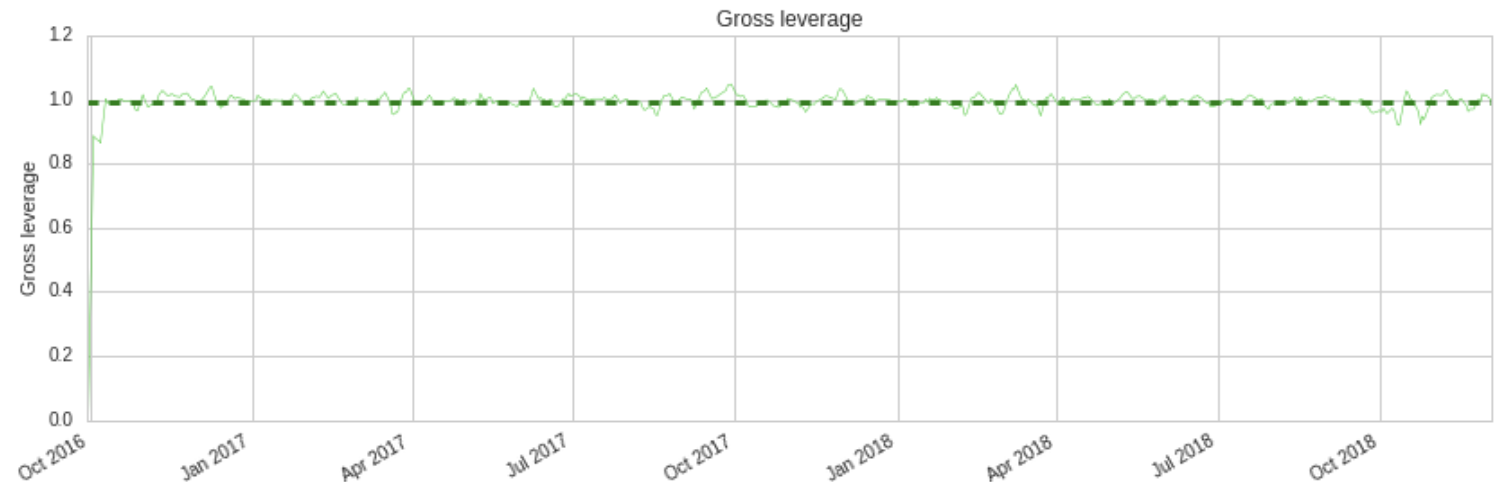
\includegraphics[width=0.8\linewidth]{/Users/jcahoon/workspace/st790-financial-stats/final/ts_leverage} 

}

\caption{\label{leverage}Gross leverage fluctuates around 1.0x as originally set in our trading algorithm.}\label{fig:unnamed-chunk-10}
\end{figure}

\begin{figure}

{\centering 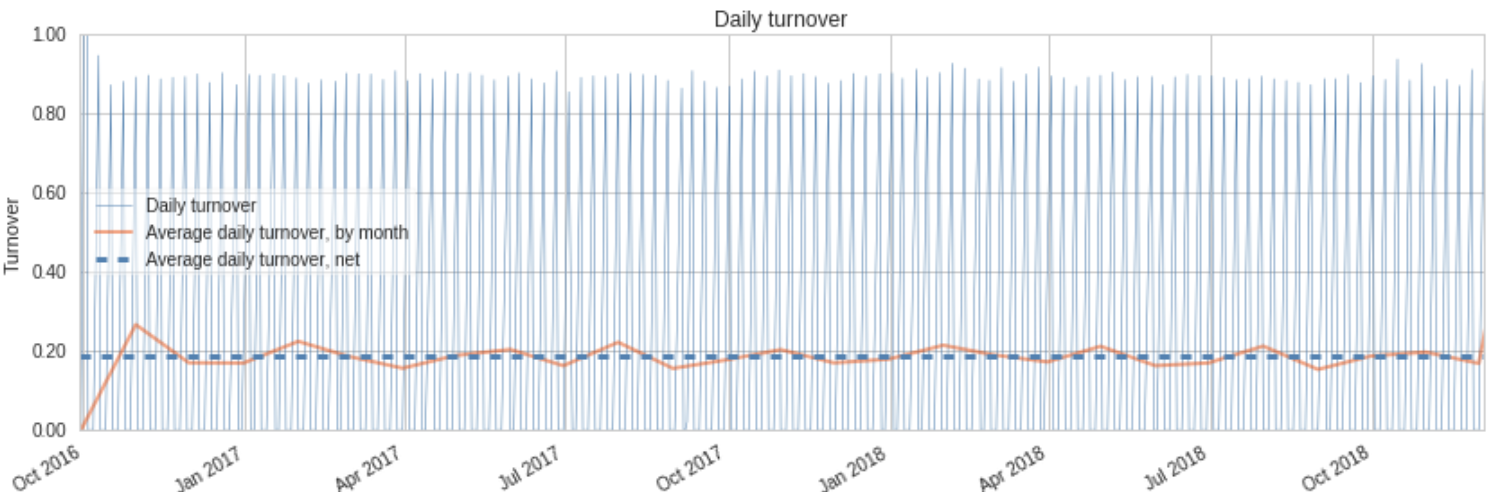
\includegraphics[width=0.8\linewidth]{/Users/jcahoon/workspace/st790-financial-stats/final/ts_dailyturnover} 

}

\caption{\label{turnover}Daily turnover of 0.80x shown weekly as originally set in our trading algorithm.}\label{fig:unnamed-chunk-11}
\end{figure}

Our original constraint of \(|w_i| < 0.05\) is also satisfied as
indicated by the top 10 long and short positions. No individual security
can have a significant impact on portfolio returns as shown in Figure
\ref{top10}. To further understand our use of our sentiment metric, we
examine the top 5 long and short stocks individually, extracting each
respective count of number of bull and bear messages assessed on
StockTwits, as well as the 5-day rolling average of its bull minus bear
intensity within our backtest window in Figure \ref{topstock} and
\ref{botstock}.

\begin{figure}

{\centering 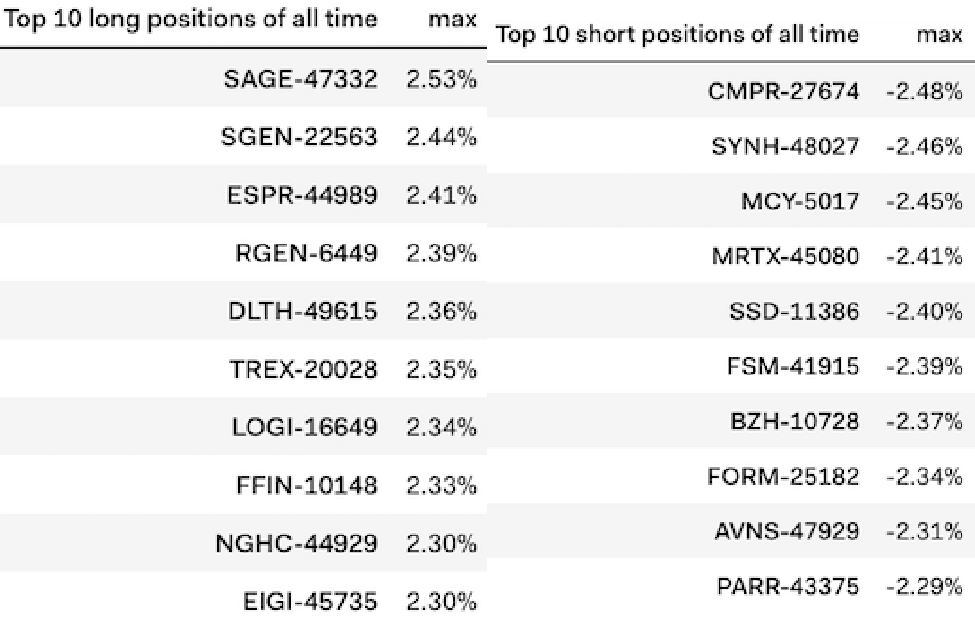
\includegraphics[width=0.6\linewidth]{cahoon_final_paper_files/figure-latex/unnamed-chunk-12-1} 

}

\caption{\label{top10}Top 10 long and short positions within the backtest period.}\label{fig:unnamed-chunk-12}
\end{figure}

\begin{figure}
\centering
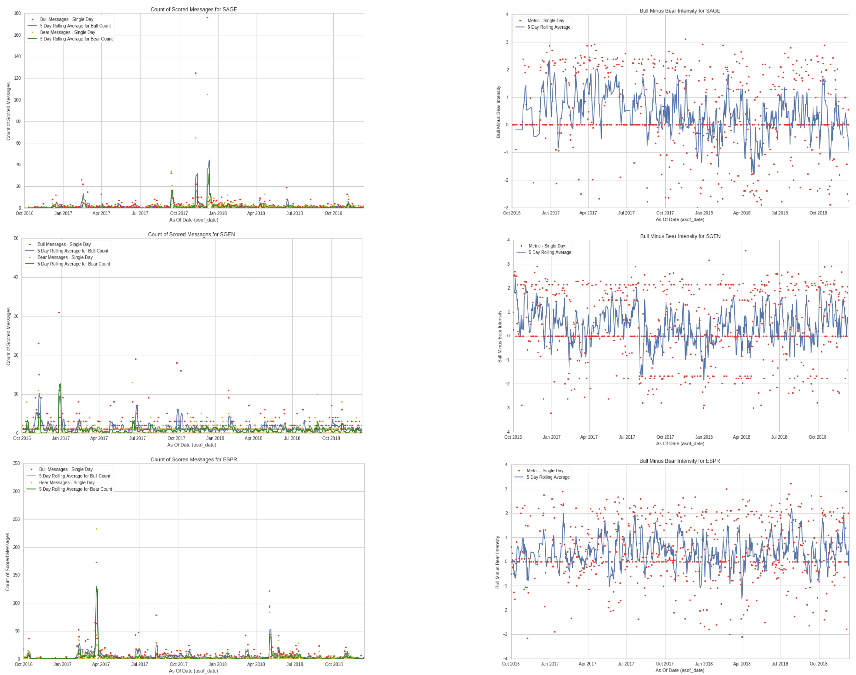
\includegraphics{cahoon_final_paper_files/figure-latex/unnamed-chunk-13-1.pdf}
\caption{\label{topstock}Raw bull and bear message counts and bull minus
bear intensities for the top 3 long positions. From top to bottom, we
have SAGE, SGEN, and ESPR shown.}
\end{figure}

\begin{figure}
\centering
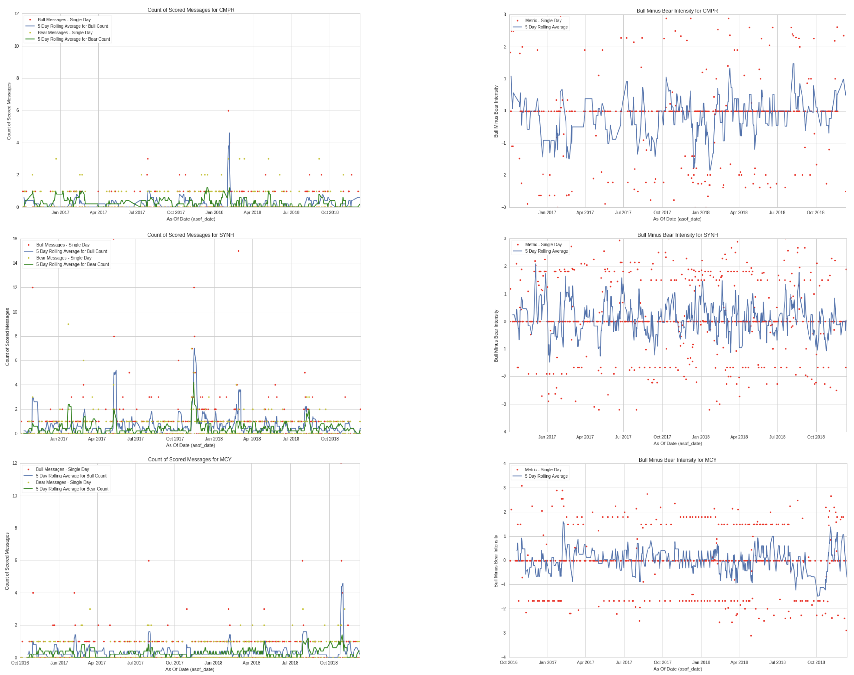
\includegraphics{cahoon_final_paper_files/figure-latex/unnamed-chunk-14-1.pdf}
\caption{\label{botstock}Raw bull and bear message counts and bull minus
bear intensities for the top 3 short positions. From top to bottom, we
have CMPR, SYNH, and MCY shown.}
\end{figure}

\hypertarget{performance}{%
\section{Performance}\label{performance}}

As shown below and alluded to earlier, our results were above average as
the overall market in November was highly volatile. Given our strategy
gets most of its returns from volatility, we were able to achieve a
relatively high score of 0.338. Moreover, we almost experienced no
drawdown despite the drawdowns in the broader US equities market. Our
final leaderboard results at the end of our one-month trading period
from November \(1^{st}\) to November \(30^{th}\) are shown in Table
\ref{leader}.

\begin{table}[ht]
\centering
\caption{Leaderboard results after the one-month trading window of November 2018}
\begin{tabular}{llr}
  \hline
 Metric & Our Result & Overall \\ 
  \hline
   rank & 105 & - \\ 
   score & 0.338 & 0.35 \\ 
   max\_beta\_to\_spy\_126day & 0.076 & 0.14 \\ 
   max\_cumulative\_common\_returns & 0.009 & 0.04 \\ 
   max\_leverage & 1.047 & 1.05 \\ 
   max\_max\_drawdown & 0.000 & -0.00 \\ 
   max\_net\_dollar\_exposure & 0.032 & 0.04 \\ 
   max\_total\_returns & 0.025 & 0.14 \\ 
   min\_total\_returns & -0.007 & -0.02 \\ 
   max\_turnover & 0.905 & 1.07 \\ 
   max\_volatility\_126day & 0.044 & 0.06 \\ 
   \hline
\end{tabular}
\label{leader}
\end{table}

\hypertarget{discussion}{%
\section{Discussion}\label{discussion}}

Closer examination of the data in Figure \ref{topstock} and
\ref{botstock} suggests that our sentiment indicator should not have
been the \emph{primary} component of our trading strategy. As shown by
the number of scored bull and bear messages in red and yellow in Figure
\ref{botstock}, the highest number of messages that were evaluated to
calculate the bull or bear intensity was less than 16. These 16 messages
appeared around February 2018 for Syneos Health (SYNH) right around when
SYNH released their positive earnings revision, resulting in a spike of
their stock price from \$35.80 to \$41.90 per share (Edward
\protect\hyperlink{ref-synh}{2018}). However, our strategy does not
trade on information within 2 days of any earnings period, so despite
StockTwits providing more text data than usual, we do not leverage this
additional information.

Unlike the top equities that we have shorted, in Figure \ref{topstock},
the bull and bear intensies are based off of a more substantial set of
StockTwits. In fact the overall bull and bear count of messages
processed for our top long equities are much higher with a max count
around 180, 30, and 250 for SAGE, SGEN, and ESPR. In general, the number
of bull messages are greater than the number of bear messages,
suggesting most users on StockTwits generally lean towards promoting
\emph{buys} rather than \emph{sells}. Moreover, we see that the peaks in
message volume are oftentimes not associated with earnings or
acquisition announcements, but other major corporate milestones. For
example, the peak in message volume for Sage Therapeutics (SAGE) occurs
around December 2017. These \textasciitilde{}180 messages can be
attributed to an announcement made by the CEO in which SAGE received
positive results after its Phase 2 trial for a drug that treats
depression (Aiello \protect\hyperlink{ref-sage1}{2017}). We can also see
a peak in message volume in the prior month of November, which can be
attributed to the successful clinicial trial results for another drug
for postpartum depression (Lovelace
\protect\hyperlink{ref-sage2}{2017}). Both of these events are marked by
high peaks in our bull minus bear intensity, providing some impetus for
the value in our sentiment metric.

In general, while our approach is market neutral and has benefitted us
during a period of high volatility in asset prices, it is too simple. We
should have adhered to ideas from literature that have shown time and
again that sentiment can be utilized to \emph{augment} a traditional
long-short equity strategy (Agrawal et al.
\protect\hyperlink{ref-agrawal2019}{2019}). Instead, our optimization
routine depended \emph{entirely} on our sentiment metric, which explains
its poor performance overall. To build on our simplistic approach, a
number of avenues we can consider include:

\begin{enumerate}
\def\labelenumi{\arabic{enumi}.}
\item
  \emph{Build a classifier from scratch}: As we have examined, the
  volume of data provided by StockTwit is not enough to fully capture
  general investor sentiment on a stock. We should attempt to build our
  own classifier from possibly richer sources of messages (e.g., Weibo,
  Twitter) that can provide a more robust measure of the bullish and
  bearish signals. Moreover, constructing our own language processing
  algorithm provides a better means to filter out noise or manipulative
  StockTwits as users each have their own agenda for making excessive
  claims about a particular asset.
\item
  \emph{Include fundamental factors}: Given the extensive literature on
  factor modeling (Fan and Yao \protect\hyperlink{ref-Fan2015}{2015}),
  we should consider leveraging these time-tested metrics and ratios,
  like market cap and book-to-price, that have captured the financial
  characteristics of an asset. We can start with the typical (i) excess
  return of small market cap minus big market cap companies, (ii) excess
  return of companies with high book-to-price against low book-to-price
  ratios, and (iii) excess return of companies that overperformed to
  those that underperformed, and study how the inclusion of these
  factors along with our sentiment index might affect returns. We might
  even find that some factors are more efficient than others, so
  swapping them in for our sentiment index might be necessary. Once we
  understand exactly how much we are exposed to specific factors, given
  the lack of predictability in the market in general, we should
  consider beta hedging to avoid any big dependencies on performance on
  a certain factor. This essentially entails taking the exposure
  \(\beta\) we have to a factor and shorting it by the proportional
  value of our total portfolio \(\beta M\).
\item
  \emph{Comprehensive exploratory data analysis}: There are basic steps
  we should have carried out prior to executing our strategy on
  Quantopian. Namely, we should have checked for normality,
  homoskedasticity, and autocorrelation in our model, as violations
  results in parameters that often biased, inconsistent and inefficient.
  If these assumptions hold, then we can actually normalize our factor
  values, allowing for them to be easily comparable across different
  asset classes. If the assumptions hold weakly, we might consider other
  transformations, like Winsorization, that will still allow us to build
  a robust statistical model for trading.
\end{enumerate}

Given some good characteristics and performance in our approach overall,
we have yet ruled out the value of using information from online
conversations like StockTwits, as a means to build a compelling
long-short US equity strategy.

\newpage

\hypertarget{appendix}{%
\section{Appendix}\label{appendix}}

\hypertarget{quantopian-submission}{%
\subsection{Quantopian Submission}\label{quantopian-submission}}

\begin{Shaded}
\begin{Highlighting}[]
\CommentTok{# Import Algorithm API functions}
\ImportTok{from}\NormalTok{ quantopian.algorithm }\ImportTok{import}\NormalTok{ (}
\NormalTok{    attach_pipeline,}
\NormalTok{    pipeline_output,}
\NormalTok{    order_optimal_portfolio,}
\NormalTok{)}
\CommentTok{# Import Optimize API module}
\ImportTok{import}\NormalTok{ quantopian.optimize }\ImportTok{as}\NormalTok{ opt}
\CommentTok{# Pipeline imports}
\ImportTok{from}\NormalTok{ quantopian.pipeline }\ImportTok{import}\NormalTok{ Pipeline}
\ImportTok{from}\NormalTok{ quantopian.pipeline.data.psychsignal }\ImportTok{import}\NormalTok{ stocktwits}
\ImportTok{from}\NormalTok{ quantopian.pipeline.factors }\ImportTok{import}\NormalTok{ SimpleMovingAverage}
\CommentTok{# Import built-in universe and Risk API method}
\ImportTok{from}\NormalTok{ quantopian.pipeline.filters }\ImportTok{import}\NormalTok{ QTradableStocksUS}
\ImportTok{from}\NormalTok{ quantopian.pipeline.experimental }\ImportTok{import}\NormalTok{ risk_loading_pipeline}
\CommentTok{# Get event data }
\ImportTok{from}\NormalTok{ quantopian.pipeline.factors.eventvestor }\ImportTok{import}\NormalTok{ (}
\NormalTok{    BusinessDaysUntilNextEarnings,}
\NormalTok{    BusinessDaysSincePreviousEarnings,}
\NormalTok{)}
\ImportTok{from}\NormalTok{ quantopian.pipeline.filters.eventvestor }\ImportTok{import}\NormalTok{ IsAnnouncedAcqTarget}
\ImportTok{from}\NormalTok{ quantopian.pipeline.factors }\ImportTok{import}\NormalTok{ BusinessDaysSincePreviousEvent}
\KeywordTok{def}\NormalTok{ initialize(context):}
    \CommentTok{# Constraint parameters}
\NormalTok{    context.max_leverage }\OperatorTok{=} \FloatTok{1.0}
\NormalTok{    context.max_pos_size }\OperatorTok{=} \FloatTok{0.05}
\NormalTok{    context.max_turnover }\OperatorTok{=} \FloatTok{0.8}
    \CommentTok{# Attach data pipelines}
\NormalTok{    attach_pipeline(}
\NormalTok{        make_pipeline(),}
        \StringTok{'data_pipe'}
\NormalTok{    )}
\NormalTok{    attach_pipeline(}
\NormalTok{        risk_loading_pipeline(),}
        \StringTok{'risk_pipe'}
\NormalTok{    )}
    \CommentTok{# Schedule rebalance function}
\NormalTok{    schedule_function(}
\NormalTok{        rebalance,}
\NormalTok{        date_rules.week_start(),}
\NormalTok{        time_rules.market_open(),}
\NormalTok{    )}
\KeywordTok{def}\NormalTok{ before_trading_start(context, data):}
    \CommentTok{# Get pipeline outputs and}
    \CommentTok{# store them in context}
\NormalTok{    context.output }\OperatorTok{=}\NormalTok{ pipeline_output(}\StringTok{'data_pipe'}\NormalTok{)}
\NormalTok{    context.risk_factor_betas }\OperatorTok{=}\NormalTok{ pipeline_output(}\StringTok{'risk_pipe'}\NormalTok{)}
\CommentTok{# Pipeline definition}
\KeywordTok{def}\NormalTok{ make_pipeline():}
   
\NormalTok{    not_near_earnings }\OperatorTok{=} \OperatorTok{~}\NormalTok{((BusinessDaysUntilNextEarnings() }\OperatorTok{<=} \DecValTok{2}\NormalTok{) }\OperatorTok{|}
\NormalTok{      (BusinessDaysSincePreviousEarnings() }\OperatorTok{<=} \DecValTok{2}\NormalTok{)) }
    
\NormalTok{    not_acq_tar }\OperatorTok{=} \OperatorTok{~}\NormalTok{IsAnnouncedAcqTarget()}
    
\NormalTok{    universe }\OperatorTok{=}\NormalTok{ (}
\NormalTok{        QTradableStocksUS()}
        \OperatorTok{&}\NormalTok{ not_near_earnings}
        \OperatorTok{&}\NormalTok{ not_acq_tar}
\NormalTok{    )}
    
\NormalTok{    sentiment_score }\OperatorTok{=}\NormalTok{ SimpleMovingAverage(}
\NormalTok{        inputs}\OperatorTok{=}\NormalTok{[stocktwits.bull_minus_bear],}
\NormalTok{        window_length}\OperatorTok{=}\DecValTok{5}\NormalTok{,}
\NormalTok{        mask}\OperatorTok{=}\NormalTok{universe}
\NormalTok{    )}
    \ControlFlowTok{return}\NormalTok{ Pipeline(}
\NormalTok{        columns}\OperatorTok{=}\NormalTok{\{}
            \StringTok{'sentiment_score'}\NormalTok{: sentiment_score,}
\NormalTok{        \},}
\NormalTok{        screen}\OperatorTok{=}\NormalTok{sentiment_score.notnull()}
\NormalTok{    )}
\KeywordTok{def}\NormalTok{ rebalance(context, data):}
    \CommentTok{# Create MaximizeAlpha objective using}
    \CommentTok{# sentiment_score data from pipeline output}
\NormalTok{    objective }\OperatorTok{=}\NormalTok{ opt.MaximizeAlpha(}
\NormalTok{      context.output.sentiment_score}
\NormalTok{    )}
    \CommentTok{# Create position size constraint}
\NormalTok{    constrain_pos_size }\OperatorTok{=}\NormalTok{ opt.PositionConcentration.with_equal_bounds(}
        \OperatorTok{-}\NormalTok{context.max_pos_size,}
\NormalTok{        context.max_pos_size}
\NormalTok{    )}
    \CommentTok{# Constrain target portfolio's leverage}
\NormalTok{    max_leverage }\OperatorTok{=}\NormalTok{ opt.MaxGrossExposure(context.max_leverage)}
    \CommentTok{# Constrain portfolio turnover}
\NormalTok{    max_turnover }\OperatorTok{=}\NormalTok{ opt.MaxTurnover(context.max_turnover)}
    \CommentTok{# Constrain target portfolio's risk exposure}
\NormalTok{    factor_risk_constraints }\OperatorTok{=}\NormalTok{ opt.experimental.RiskModelExposure(}
\NormalTok{        context.risk_factor_betas,}
\NormalTok{        version}\OperatorTok{=}\NormalTok{opt.Newest}
\NormalTok{    )}
    \CommentTok{# Rebalance portfolio using objective}
    \CommentTok{# and list of constraints}
\NormalTok{    order_optimal_portfolio(}
\NormalTok{        objective}\OperatorTok{=}\NormalTok{objective,}
\NormalTok{        constraints}\OperatorTok{=}\NormalTok{[}
\NormalTok{            max_leverage,}
\NormalTok{            constrain_pos_size,}
\NormalTok{            max_turnover,}
\NormalTok{            factor_risk_constraints,}
\NormalTok{        ]}
\NormalTok{    )}
\end{Highlighting}
\end{Shaded}

\hypertarget{data-exploration}{%
\subsection{Data Exploration}\label{data-exploration}}

\begin{Shaded}
\begin{Highlighting}[]
\CommentTok{# Import the free sample of the dataset}
\ImportTok{from}\NormalTok{ quantopian.interactive.data.psychsignal }\ImportTok{import}\NormalTok{ stocktwits_free  }\ImportTok{as}\NormalTok{ dataset}
\CommentTok{# Import data operations}
\ImportTok{from}\NormalTok{ odo }\ImportTok{import}\NormalTok{ odo}
\CommentTok{# Import other libraries}
\ImportTok{import}\NormalTok{ pandas }\ImportTok{as}\NormalTok{ pd}
\ImportTok{import}\NormalTok{ matplotlib.pyplot }\ImportTok{as}\NormalTok{ plt}
\ImportTok{import}\NormalTok{ datetime }\ImportTok{as}\NormalTok{ dt}
\CommentTok{# Filtering for an equity (here SSD)}
\NormalTok{ssd }\OperatorTok{=}\NormalTok{ dataset[dataset.sid }\OperatorTok{==} \DecValTok{11386}\NormalTok{] }\CommentTok{# aapl is 24}
\NormalTok{ssd_df }\OperatorTok{=}\NormalTok{ odo(ssd.sort(}\StringTok{'asof_date'}\NormalTok{), pd.DataFrame)}
\NormalTok{ssd_df2 }\OperatorTok{=}\NormalTok{ ssd_df[ssd_df.asof_date }\OperatorTok{>=}\NormalTok{ dt.date(}\DecValTok{2016}\NormalTok{, }\DecValTok{9}\NormalTok{, }\DecValTok{30}\NormalTok{)]}
\NormalTok{plt.plot(ssd_df2.asof_date, ssd_df2.bull_scored_messages, marker}\OperatorTok{=}\StringTok{'.'}\NormalTok{, linestyle}\OperatorTok{=}\StringTok{'None'}\NormalTok{, color}\OperatorTok{=}\StringTok{'r'}\NormalTok{)}
\NormalTok{plt.plot(ssd_df2.asof_date, ssd_df2.bull_scored_messages.rolling(window }\OperatorTok{=} \DecValTok{5}\NormalTok{, center }\OperatorTok{=} \VariableTok{False}\NormalTok{).mean())}
\NormalTok{plt.plot(ssd_df2.asof_date, ssd_df2.bear_scored_messages, marker}\OperatorTok{=}\StringTok{'.'}\NormalTok{, linestyle}\OperatorTok{=}\StringTok{'None'}\NormalTok{, color}\OperatorTok{=}\StringTok{'y'}\NormalTok{)}
\NormalTok{plt.plot(ssd_df2.asof_date, ssd_df2.bear_scored_messages.rolling(window }\OperatorTok{=} \DecValTok{5}\NormalTok{, center }\OperatorTok{=} \VariableTok{False}\NormalTok{).mean(), color}\OperatorTok{=}\StringTok{'g'}\NormalTok{)}
\NormalTok{plt.xlabel(}\StringTok{"As Of Date (asof_date)"}\NormalTok{)}
\NormalTok{plt.ylabel(}\StringTok{"Count of Scored Messages"}\NormalTok{)}
\NormalTok{plt.title(}\StringTok{"Count of Scored Messages for SSD"}\NormalTok{)}
\NormalTok{plt.legend([}\StringTok{"Bull Messages - Single Day"}\NormalTok{, }\StringTok{"5 Day Rolling Average for Bull Count"}\NormalTok{, }\StringTok{"Bear Messages - Single Day"}\NormalTok{, }\StringTok{"5 Day Rolling Average for Bear Count"}\NormalTok{], loc}\OperatorTok{=}\DecValTok{2}\NormalTok{)}
\NormalTok{plt.plot(ssd_df2.asof_date, ssd_df2.bull_minus_bear, marker}\OperatorTok{=}\StringTok{'.'}\NormalTok{, linestyle}\OperatorTok{=}\StringTok{'None'}\NormalTok{, color}\OperatorTok{=}\StringTok{'r'}\NormalTok{)}
\NormalTok{plt.plot(ssd_df2.asof_date, ssd_df2.bull_minus_bear.rolling(window }\OperatorTok{=} \DecValTok{5}\NormalTok{, center }\OperatorTok{=} \VariableTok{False}\NormalTok{).mean())}
\NormalTok{plt.xlabel(}\StringTok{"As Of Date (asof_date)"}\NormalTok{)}
\NormalTok{plt.ylabel(}\StringTok{"Bull Minus Bear Intensity"}\NormalTok{)}
\NormalTok{plt.title(}\StringTok{"Bull Minus Bear Intensity for SSD"}\NormalTok{)}
\NormalTok{plt.legend([}\StringTok{"Metric - Single Day"}\NormalTok{, }\StringTok{"5 Day Rolling Average"}\NormalTok{], loc}\OperatorTok{=}\DecValTok{2}\NormalTok{)}
\end{Highlighting}
\end{Shaded}

\hypertarget{factor-analysis}{%
\subsection{Factor Analysis}\label{factor-analysis}}

\begin{Shaded}
\begin{Highlighting}[]
\ImportTok{from}\NormalTok{ quantopian.pipeline }\ImportTok{import}\NormalTok{ Pipeline}
\ImportTok{from}\NormalTok{ quantopian.research }\ImportTok{import}\NormalTok{ run_pipeline}
\ImportTok{from}\NormalTok{ quantopian.pipeline.factors }\ImportTok{import}\NormalTok{ SimpleMovingAverage}
\ImportTok{from}\NormalTok{ quantopian.pipeline.factors }\ImportTok{import}\NormalTok{ CustomFactor}
\ImportTok{from}\NormalTok{ quantopian.pipeline.filters }\ImportTok{import}\NormalTok{ Q1500US}
\ImportTok{from}\NormalTok{ quantopian.pipeline.filters }\ImportTok{import}\NormalTok{ QTradableStocksUS}
\ImportTok{from}\NormalTok{ quantopian.pipeline.classifiers.morningstar }\ImportTok{import}\NormalTok{ Sector}
\ImportTok{from}\NormalTok{ quantopian.pipeline.data.builtin }\ImportTok{import}\NormalTok{ USEquityPricing}
\ImportTok{from}\NormalTok{ quantopian.pipeline.data.psychsignal }\ImportTok{import}\NormalTok{ stocktwits}
\ImportTok{from}\NormalTok{ quantopian.research.experimental }\ImportTok{import}\NormalTok{ get_factor_returns, get_factor_loadings}
\ImportTok{import}\NormalTok{ alphalens }\ImportTok{as}\NormalTok{ al}
\ImportTok{import}\NormalTok{ numpy }\ImportTok{as}\NormalTok{ np}
\ImportTok{import}\NormalTok{ pandas }\ImportTok{as}\NormalTok{ pd}
\ImportTok{import}\NormalTok{ matplotlib.pyplot }\ImportTok{as}\NormalTok{ plt}
\ImportTok{import}\NormalTok{ seaborn }\ImportTok{as}\NormalTok{ sns}
\ImportTok{import}\NormalTok{ empyrical }\ImportTok{as}\NormalTok{ ep}
\ImportTok{import}\NormalTok{ alphalens }\ImportTok{as}\NormalTok{ al}
\ImportTok{import}\NormalTok{ pyfolio }\ImportTok{as}\NormalTok{ pf}
\NormalTok{universe }\OperatorTok{=}\NormalTok{ QTradableStocksUS()}
\NormalTok{pipeline_factor }\OperatorTok{=}\NormalTok{ SimpleMovingAverage(}
\NormalTok{    inputs}\OperatorTok{=}\NormalTok{[stocktwits.bull_minus_bear], }
\NormalTok{    window_length}\OperatorTok{=}\DecValTok{5}\NormalTok{)}
\NormalTok{pipe }\OperatorTok{=}\NormalTok{ Pipeline(screen}\OperatorTok{=}\NormalTok{universe, columns}\OperatorTok{=}\NormalTok{\{}\StringTok{'alpha'}\NormalTok{: pipeline_factor\})}
\KeywordTok{def}\NormalTok{ compute_specific_returns(total_returns, factor_returns}\OperatorTok{=}\VariableTok{None}\NormalTok{, factor_loadings}\OperatorTok{=}\VariableTok{None}\NormalTok{, assets}\OperatorTok{=}\VariableTok{None}\NormalTok{):}
    \ControlFlowTok{if}\NormalTok{ assets }\KeywordTok{is} \KeywordTok{not} \VariableTok{None}\NormalTok{:}
\NormalTok{        factor_loadings }\OperatorTok{=}\NormalTok{ get_factor_loadings(assets, start, end }\OperatorTok{+}\NormalTok{ pd.Timedelta(days}\OperatorTok{=}\DecValTok{30}\NormalTok{))}
\NormalTok{        factor_returns }\OperatorTok{=}\NormalTok{ get_factor_returns(start, end }\OperatorTok{+}\NormalTok{ pd.Timedelta(days}\OperatorTok{=}\DecValTok{30}\NormalTok{))}
    \ControlFlowTok{elif}\NormalTok{ factor_loadings }\KeywordTok{is} \VariableTok{None} \KeywordTok{or}\NormalTok{ factor_returns }\KeywordTok{is} \VariableTok{None}\NormalTok{:}
        \ControlFlowTok{raise} \PreprocessorTok{ValueError}\NormalTok{(}\StringTok{'Supply either assets or factor_returns and factor_loadings'}\NormalTok{)}
    
\NormalTok{    factor_returns.index }\OperatorTok{=}\NormalTok{ factor_returns.index.set_names([}\StringTok{'dt'}\NormalTok{])}
\NormalTok{    factor_loadings.index }\OperatorTok{=}\NormalTok{ factor_loadings.index.set_names([}\StringTok{'dt'}\NormalTok{, }\StringTok{'ticker'}\NormalTok{])}
\NormalTok{    common_returns }\OperatorTok{=}\NormalTok{ factor_loadings.mul(factor_returns).}\BuiltInTok{sum}\NormalTok{(axis}\OperatorTok{=}\StringTok{'columns'}\NormalTok{).unstack()}
\NormalTok{    specific_returns }\OperatorTok{=}\NormalTok{ total_returns }\OperatorTok{-}\NormalTok{ common_returns}
    \ControlFlowTok{return}\NormalTok{ specific_returns}
\KeywordTok{def}\NormalTok{ factor_portfolio_returns(factor, pricing, equal_weight}\OperatorTok{=}\VariableTok{True}\NormalTok{, delay}\OperatorTok{=}\DecValTok{0}\NormalTok{):}
    \ControlFlowTok{if}\NormalTok{ equal_weight:}
\NormalTok{        factor }\OperatorTok{=}\NormalTok{ np.sign(results[}\StringTok{'alpha'}\NormalTok{])}
\NormalTok{        bins }\OperatorTok{=}\NormalTok{ (}\OperatorTok{-}\DecValTok{1}\NormalTok{, }\DecValTok{0}\NormalTok{, }\DecValTok{1}\NormalTok{)}
\NormalTok{        quantiles }\OperatorTok{=} \VariableTok{None}
\NormalTok{        zero_aware }\OperatorTok{=} \VariableTok{False}
    \ControlFlowTok{else}\NormalTok{:}
\NormalTok{        bins }\OperatorTok{=} \VariableTok{None}
\NormalTok{        quantiles }\OperatorTok{=} \DecValTok{5}
\NormalTok{        zero_aware }\OperatorTok{=} \VariableTok{True}
        
\NormalTok{    pos }\OperatorTok{=}\NormalTok{ factor.unstack().fillna(}\DecValTok{0}\NormalTok{)}
\NormalTok{    pos }\OperatorTok{=}\NormalTok{ (pos }\OperatorTok{/}\NormalTok{ pos.}\BuiltInTok{abs}\NormalTok{().}\BuiltInTok{sum}\NormalTok{()).reindex(pricing.index).ffill().shift(delay)}
    \CommentTok{# Fully invested, shorts show up as cash}
\NormalTok{    pos[}\StringTok{'cash'}\NormalTok{] }\OperatorTok{=}\NormalTok{ pos[pos }\OperatorTok{<} \DecValTok{0}\NormalTok{].}\BuiltInTok{sum}\NormalTok{(axis}\OperatorTok{=}\StringTok{'columns'}\NormalTok{)}
    
\NormalTok{    factor_and_returns }\OperatorTok{=}\NormalTok{ al.utils.get_clean_factor_and_forward_returns(}
\NormalTok{        pos.stack().loc[}\KeywordTok{lambda}\NormalTok{ x: x }\OperatorTok{!=} \DecValTok{0}\NormalTok{], }
\NormalTok{        pricing, periods}\OperatorTok{=}\NormalTok{(}\DecValTok{1}\NormalTok{,), quantiles}\OperatorTok{=}\NormalTok{quantiles, bins}\OperatorTok{=}\NormalTok{bins, }
\NormalTok{        zero_aware}\OperatorTok{=}\NormalTok{zero_aware)}
    
    \ControlFlowTok{return}\NormalTok{ al.performance.factor_returns(factor_and_returns)[}\StringTok{'1D'}\NormalTok{], pos}
\KeywordTok{def}\NormalTok{ plot_ic_over_time(factor_data, label}\OperatorTok{=}\StringTok{''}\NormalTok{, ax}\OperatorTok{=}\VariableTok{None}\NormalTok{):}
\NormalTok{    mic }\OperatorTok{=}\NormalTok{ al.performance.mean_information_coefficient(factor_data)}
\NormalTok{    mic.index }\OperatorTok{=}\NormalTok{ mic.index.}\BuiltInTok{map}\NormalTok{(}\KeywordTok{lambda}\NormalTok{ x: }\BuiltInTok{int}\NormalTok{(x[:}\OperatorTok{-}\DecValTok{1}\NormalTok{])) }
\NormalTok{    ax }\OperatorTok{=}\NormalTok{ mic.plot(label}\OperatorTok{=}\NormalTok{label, ax}\OperatorTok{=}\NormalTok{ax)}
\NormalTok{    ax.}\BuiltInTok{set}\NormalTok{(xlabel}\OperatorTok{=}\StringTok{'Days'}\NormalTok{, ylabel}\OperatorTok{=}\StringTok{'Mean IC'}\NormalTok{)}
\NormalTok{    ax.legend()}
\NormalTok{    ax.axhline(}\DecValTok{0}\NormalTok{, ls}\OperatorTok{=}\StringTok{'--'}\NormalTok{, color}\OperatorTok{=}\StringTok{'k'}\NormalTok{)}
    
\KeywordTok{def}\NormalTok{ plot_cum_returns_delay(factor, pricing, delay}\OperatorTok{=}\BuiltInTok{range}\NormalTok{(}\DecValTok{5}\NormalTok{), ax}\OperatorTok{=}\VariableTok{None}\NormalTok{):}
    \ControlFlowTok{if}\NormalTok{ ax }\KeywordTok{is} \VariableTok{None}\NormalTok{:}
\NormalTok{        fig, ax }\OperatorTok{=}\NormalTok{ plt.subplots()}
    \ControlFlowTok{for}\NormalTok{ d }\KeywordTok{in}\NormalTok{ delay:}
\NormalTok{        portfolio_returns, _ }\OperatorTok{=}\NormalTok{ factor_portfolio_returns(results[}\StringTok{'alpha'}\NormalTok{], pricing, delay}\OperatorTok{=}\NormalTok{d)}
\NormalTok{        ep.cum_returns(portfolio_returns).plot(ax}\OperatorTok{=}\NormalTok{ax, label}\OperatorTok{=}\NormalTok{d)}
\NormalTok{    ax.legend()}
\NormalTok{    ax.}\BuiltInTok{set}\NormalTok{(ylabel}\OperatorTok{=}\StringTok{'Cumulative returns'}\NormalTok{, title}\OperatorTok{=}\StringTok{'Cumulative returns if factor is delayed'}\NormalTok{)}
    
\KeywordTok{def}\NormalTok{ plot_exposures(risk_exposures, ax}\OperatorTok{=}\VariableTok{None}\NormalTok{):}
\NormalTok{    rep }\OperatorTok{=}\NormalTok{ risk_exposures.stack().reset_index()}
\NormalTok{    rep.columns }\OperatorTok{=}\NormalTok{ [}\StringTok{'dt'}\NormalTok{, }\StringTok{'factor'}\NormalTok{, }\StringTok{'exposure'}\NormalTok{]}
\NormalTok{    sns.boxplot(x}\OperatorTok{=}\StringTok{'exposure'}\NormalTok{, y}\OperatorTok{=}\StringTok{'factor'}\NormalTok{, data}\OperatorTok{=}\NormalTok{rep, orient}\OperatorTok{=}\StringTok{'h'}\NormalTok{, ax}\OperatorTok{=}\NormalTok{ax, order}\OperatorTok{=}\NormalTok{risk_exposures.columns[::}\OperatorTok{-}\DecValTok{1}\NormalTok{])}
    
\KeywordTok{def}\NormalTok{ plot_overview_tear_sheet(factor, prices, factor_returns, factor_loadings, periods}\OperatorTok{=}\BuiltInTok{range}\NormalTok{(}\DecValTok{1}\NormalTok{, }\DecValTok{15}\NormalTok{)):}
\NormalTok{    stock_rets }\OperatorTok{=}\NormalTok{ pricing.pct_change()}
\NormalTok{    stock_rets_specific }\OperatorTok{=}\NormalTok{ compute_specific_returns(stock_rets, factor_returns, factor_loadings)}
\NormalTok{    cr_specific }\OperatorTok{=}\NormalTok{ ep.cum_returns(stock_rets_specific, starting_value}\OperatorTok{=}\DecValTok{1}\NormalTok{)}
    
\NormalTok{    factor_data_total }\OperatorTok{=}\NormalTok{ al.utils.get_clean_factor_and_forward_returns(}
\NormalTok{        factor, }
\NormalTok{        pricing)}
    
\NormalTok{    factor_data_specific }\OperatorTok{=}\NormalTok{ al.utils.get_clean_factor_and_forward_returns(}
\NormalTok{        factor, }
\NormalTok{        cr_specific)}
    
\NormalTok{    portfolio_returns, portfolio_pos }\OperatorTok{=}\NormalTok{ factor_portfolio_returns(factor, pricing)}
\NormalTok{    factor_loadings.index }\OperatorTok{=}\NormalTok{ factor_loadings.index.set_names([}\StringTok{'dt'}\NormalTok{, }\StringTok{'ticker'}\NormalTok{])}
\NormalTok{    portfolio_pos.index }\OperatorTok{=}\NormalTok{ portfolio_pos.index.set_names([}\StringTok{'dt'}\NormalTok{])}
\NormalTok{    risk_exposures_portfolio, perf_attribution }\OperatorTok{=}\NormalTok{ pf.perf_attrib.perf_attrib(}
\NormalTok{        portfolio_returns, }
\NormalTok{        portfolio_pos, }
\NormalTok{        factor_returns, }
\NormalTok{        factor_loadings, }
\NormalTok{        pos_in_dollars}\OperatorTok{=}\VariableTok{False}\NormalTok{)}
\NormalTok{    fig }\OperatorTok{=}\NormalTok{ plt.figure(figsize}\OperatorTok{=}\NormalTok{(}\DecValTok{16}\NormalTok{, }\DecValTok{16}\NormalTok{))}
\NormalTok{    gs }\OperatorTok{=}\NormalTok{ plt.GridSpec(}\DecValTok{4}\NormalTok{, }\DecValTok{4}\NormalTok{)}
\NormalTok{    ax1 }\OperatorTok{=}\NormalTok{ plt.subplot(gs[}\DecValTok{0}\NormalTok{:}\DecValTok{2}\NormalTok{, }\DecValTok{0}\NormalTok{:}\DecValTok{2}\NormalTok{])}
\NormalTok{    plot_ic_over_time(factor_data_total, label}\OperatorTok{=}\StringTok{'Total returns'}\NormalTok{, ax}\OperatorTok{=}\NormalTok{ax1)}
 
\NormalTok{    ax2 }\OperatorTok{=}\NormalTok{ plt.subplot(gs[}\DecValTok{0}\NormalTok{:}\DecValTok{2}\NormalTok{, }\DecValTok{2}\NormalTok{:}\DecValTok{4}\NormalTok{])}
\NormalTok{    plot_cum_returns_delay(factor, pricing, ax}\OperatorTok{=}\NormalTok{ax2)}
\NormalTok{    ax3 }\OperatorTok{=}\NormalTok{ plt.subplot(gs[}\DecValTok{2}\NormalTok{:}\DecValTok{4}\NormalTok{, }\DecValTok{0}\NormalTok{:}\DecValTok{2}\NormalTok{])}
\NormalTok{    plot_exposures(risk_exposures_portfolio.reindex(columns}\OperatorTok{=}\NormalTok{perf_attribution.columns), }
\NormalTok{                   ax}\OperatorTok{=}\NormalTok{ax3)}
\NormalTok{    ax4 }\OperatorTok{=}\NormalTok{ plt.subplot(gs[}\DecValTok{2}\NormalTok{:}\DecValTok{4}\NormalTok{, }\DecValTok{2}\NormalTok{])}
\NormalTok{    ep.cum_returns_final(perf_attribution).plot.barh(ax}\OperatorTok{=}\NormalTok{ax4)}
\NormalTok{    ax4.}\BuiltInTok{set}\NormalTok{(xlabel}\OperatorTok{=}\StringTok{'Cumulative returns'}\NormalTok{)}
\NormalTok{    ax5 }\OperatorTok{=}\NormalTok{ plt.subplot(gs[}\DecValTok{2}\NormalTok{:}\DecValTok{4}\NormalTok{, }\DecValTok{3}\NormalTok{], sharey}\OperatorTok{=}\NormalTok{ax4)}
\NormalTok{    perf_attribution.}\BuiltInTok{apply}\NormalTok{(ep.annual_volatility).plot.barh(ax}\OperatorTok{=}\NormalTok{ax5, color}\OperatorTok{=}\StringTok{'r'}\NormalTok{)}
\NormalTok{    ax5.}\BuiltInTok{set}\NormalTok{(xlabel}\OperatorTok{=}\StringTok{'Ann. volatility'}\NormalTok{)}
\NormalTok{    gs.tight_layout(fig)}
    
\NormalTok{start }\OperatorTok{=}\NormalTok{ pd.Timestamp(}\StringTok{"2018-01-01"}\NormalTok{)}
\NormalTok{end }\OperatorTok{=}\NormalTok{ pd.Timestamp(}\StringTok{"2018-10-01"}\NormalTok{)}
\NormalTok{results }\OperatorTok{=}\NormalTok{ run_pipeline(pipe, start_date}\OperatorTok{=}\NormalTok{start, end_date}\OperatorTok{=}\NormalTok{end).dropna()}
\NormalTok{assets }\OperatorTok{=}\NormalTok{ results.index.levels[}\DecValTok{1}\NormalTok{]}
\NormalTok{pricing }\OperatorTok{=}\NormalTok{ get_pricing(assets, start, end }\OperatorTok{+}\NormalTok{ pd.Timedelta(days}\OperatorTok{=}\DecValTok{30}\NormalTok{), fields}\OperatorTok{=}\StringTok{"close_price"}\NormalTok{)}
\CommentTok{# Load risk factor loadings and returns}
\NormalTok{factor_loadings }\OperatorTok{=}\NormalTok{ get_factor_loadings(assets, start, end }\OperatorTok{+}\NormalTok{ pd.Timedelta(days}\OperatorTok{=}\DecValTok{30}\NormalTok{))}
\NormalTok{factor_returns }\OperatorTok{=}\NormalTok{ get_factor_returns(start, end }\OperatorTok{+}\NormalTok{ pd.Timedelta(days}\OperatorTok{=}\DecValTok{30}\NormalTok{))}
\NormalTok{plot_overview_tear_sheet(results[}\StringTok{'alpha'}\NormalTok{], pricing, factor_returns, factor_loadings)}
\end{Highlighting}
\end{Shaded}

\hypertarget{references}{%
\section*{References}\label{references}}
\addcontentsline{toc}{section}{References}

\hypertarget{refs}{}
\leavevmode\hypertarget{ref-agrawal2019}{}%
Agrawal, S., Azar, P., Lo, A., and Singh, T. (2019), ``Practical
applications of momentum, mean-reversion, and social media: Evidence
from stocktwits and twitter,'' \emph{Practical Applications},
Institutional Investor Journals Umbrella, 6, 1--4.

\leavevmode\hypertarget{ref-sage1}{}%
Aiello, C. (2017), ``Sage ceo hopes experimental depression drug will be
as big as prozac,''
\url{https://www.cnbc.com/2017/12/08/sage-ceo-hopes-experimental-depression-drug-as-big-as-prozac-104888278.html}.

\leavevmode\hypertarget{ref-antweiler2004}{}%
Antweiler, W., and Frank, M. (2004), ``Is all that talk just noise? The
information content of internet stock message boards,'' \emph{The
Journal of finance}, Wiley Online Library, 59, 1259--1294.

\leavevmode\hypertarget{ref-bagnoli1999}{}%
Bagnoli, M., Beneish, M., and Watts, S. (1999), ``Whisper forecasts of
quarterly earnings per share,'' \emph{Journal of Accounting and
Economics}, Elsevier, 28, 27--50.

\leavevmode\hypertarget{ref-cutler1988}{}%
Cutler, D., Poterba, J., and Summers, L. (1988), ``What moves stock
prices?'' National Bureau of Economic Research.

\leavevmode\hypertarget{ref-das2007}{}%
Das, S., and Chen, M. (2007), ``Yahoo! For amazon: Sentiment extraction
from small talk on the web,'' \emph{Management science}, INFORMS, 53,
1375--1388.

\leavevmode\hypertarget{ref-dewally2003}{}%
Dewally, M. (2003), ``Internet investment advice: Investing with a rock
of salt,'' \emph{Financial Analysts Journal}, CFA Institute, 59, 65--77.

\leavevmode\hypertarget{ref-synh}{}%
Edward, A. (2018), ``Syneos health reaches a new high,''
\url{https://finreviewer.com/2018/12/11/syneos-health-inc-synh-reaches-47-64-formed-h-albireo-pharma-albo-shorts-lowered-by-9-88/}.

\leavevmode\hypertarget{ref-Fan2015}{}%
Fan, J., and Yao, Q. (2015), \emph{The elements of financial
econometrics}, Science Press.

\leavevmode\hypertarget{ref-fang2009}{}%
Fang, L., and Peress, J. (2009), ``Media coverage and the cross-section
of stock returns,'' \emph{The Journal of Finance}, Wiley Online Library,
64, 2023--2052.

\leavevmode\hypertarget{ref-cramer2018}{}%
Gurdus, E. (2018), ``Cramer: Volatility charts suggest now is the time
to buy into stocks,'' \emph{CNBC},
\url{https://www.cnbc.com/2018/11/27/cramer-volatility-charts-suggest-now-is-the-time-to-buy-into-stocks.html}.

\leavevmode\hypertarget{ref-leinweber2011}{}%
Leinweber, D., and Sisk, J. (2011), ``Event driven trading and the'new
news'.''

\leavevmode\hypertarget{ref-sage2}{}%
Lovelace, B. (2017), ``Sage therapeutics shares soar after postpartum
depression drug meets main goal,''
\url{https://www.cnbc.com/2017/11/09/sage-therapeutics-shares-soar-after-postpartum-drug-meets-main-goal.html}.

\leavevmode\hypertarget{ref-mitra2008}{}%
Mitra, L., Mitra, G., and Bartolomeo, D. (2008), ``Equity portfolio risk
(volatility) estimation using market information and sentiment,''
\emph{Quantitative Finance}.

\leavevmode\hypertarget{ref-q}{}%
Quantopian (2018), \url{https://www.quantopian.com/contest}.

\leavevmode\hypertarget{ref-st}{}%
``StockTwits'' (2018), \url{https://stocktwits.com/}.

\leavevmode\hypertarget{ref-tetlock2007}{}%
Tetlock, P. (2007), ``Giving content to investor sentiment: The role of
media in the stock market,'' \emph{The Journal of finance}, Wiley Online
Library, 62, 1139--1168.

\leavevmode\hypertarget{ref-tumarkin2001}{}%
Tumarkin, R., and Whitelaw, R. (2001), ``News or noise? Internet
postings and stock prices,'' \emph{Financial Analysts Journal}, CFA
Institute, 57, 41--51.

\leavevmode\hypertarget{ref-wysocki1998}{}%
Wysocki, P. (1998), ``Cheap talk on the web: The determinants of
postings on stock message boards.''


\end{document}
